\documentclass[aspectratio=169]{beamer}

\usetheme{Boadilla}
\usefonttheme{professionalfonts}
\setbeamertemplate{navigation symbols}{}
\setbeamertemplate{itemize items}[circle]
\setbeamertemplate{enumerate items}[default]
\setbeamertemplate{headline}{}

\usepackage[utf8]{inputenc}
\usepackage[T1]{fontenc}
\usepackage{lmodern}
\usepackage{amsmath}
\usepackage{booktabs}
\usepackage{tabularx}
\usepackage{array}
\usepackage{hyperref}
\usepackage[strings]{underscore}
\usepackage{listings}
\usepackage{tikz}
\usetikzlibrary{arrows.meta,positioning,fit,calc,shapes.geometric}
\usepackage{xcolor}

\definecolor{courseblue}{HTML}{12355B}
\definecolor{coursegold}{HTML}{C98A2E}
\definecolor{courseice}{HTML}{EEF3F8}
\definecolor{coursegreen}{HTML}{2F6B4F}
\definecolor{coursegray}{HTML}{4B5563}
\definecolor{codebg}{HTML}{F7F9FC}
\definecolor{codecomment}{HTML}{5E6C84}
\definecolor{codestring}{HTML}{0B6E4F}

\setbeamercolor{palette primary}{bg=courseblue,fg=white}
\setbeamercolor{palette secondary}{bg=coursegold,fg=white}
\setbeamercolor{palette tertiary}{bg=courseblue,fg=white}
\setbeamercolor{palette quaternary}{bg=coursegold,fg=white}
\setbeamercolor{structure}{fg=courseblue}
\setbeamercolor{frametitle}{bg=courseice,fg=courseblue}
\setbeamercolor{title}{fg=courseblue}
\setbeamercolor{block title}{bg=courseblue,fg=white}
\setbeamercolor{block body}{bg=courseice,fg=black}
\setbeamercolor{normal text}{fg=black,bg=white}
\setbeamercolor{alerted text}{fg=coursegold}

\setbeamerfont{footline}{size=\scriptsize}

\setbeamertemplate{footline}{
  \leavevmode
  \hbox{
    \begin{beamercolorbox}[wd=.33\paperwidth,ht=2.8ex,dp=1.2ex,leftskip=0.8em]{palette primary}%
      University of Trieste
    \end{beamercolorbox}%
    \begin{beamercolorbox}[wd=.49\paperwidth,ht=2.8ex,dp=1.2ex,center]{palette tertiary}%
      \coursename{} \textbar{} \coursecode
    \end{beamercolorbox}%
    \begin{beamercolorbox}[wd=.18\paperwidth,ht=2.8ex,dp=1.2ex,rightskip=0.8em plus1fil]{palette secondary}%
      \insertframenumber{} / \inserttotalframenumber
    \end{beamercolorbox}%
  }
}

\hypersetup{
  colorlinks=true,
  linkcolor=courseblue,
  urlcolor=coursegreen
}

\lstdefinestyle{coursepython}{
  language=Python,
  basicstyle=\ttfamily\footnotesize,
  keywordstyle=\color{courseblue}\bfseries,
  commentstyle=\color{codecomment}\itshape,
  stringstyle=\color{codestring},
  showstringspaces=false,
  columns=fullflexible,
  keepspaces=true,
  frame=single,
  framerule=0.6pt,
  rulecolor=\color{courseblue},
  backgroundcolor=\color{codebg},
  xleftmargin=0.4em,
  xrightmargin=0.4em,
  aboveskip=0.4em,
  belowskip=0.2em
}

\newcommand{\coursename}{Data-driven Systems Engineering}
\newcommand{\coursecode}{440MI / 305SM}
\newcommand{\coursefooter}{}

\newcommand{\learninggoals}[1]{
  \begin{block}{Learning goals}
  #1
  \end{block}
}

\newcommand{\repoactivity}[1]{
  \begin{block}{Repo activity}
  #1
  \end{block}
}

\newcommand{\readinglist}[1]{
  \begin{block}{Papers and materials}
  {\footnotesize #1}
  \end{block}
}

\newcommand{\coursecontextframe}[5]{
  \begin{frame}{Course Map and Running Cases}
  \centering
  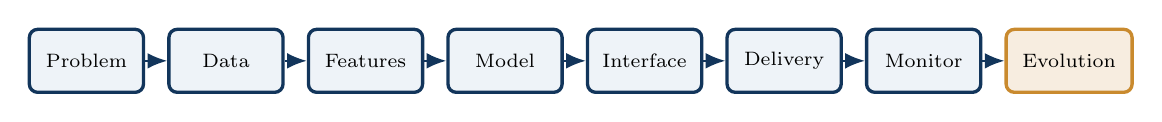
\begin{tikzpicture}[node distance=0.28cm]
  \node[flowbox, minimum width=1.45cm, minimum height=0.8cm] (problem) {\scriptsize Problem};
  \node[flowbox, minimum width=1.45cm, minimum height=0.8cm, right=of problem] (data) {\scriptsize Data};
  \node[flowbox, minimum width=1.45cm, minimum height=0.8cm, right=of data] (features) {\scriptsize Features};
  \node[flowbox, minimum width=1.45cm, minimum height=0.8cm, right=of features] (model) {\scriptsize Model};
  \node[flowbox, minimum width=1.45cm, minimum height=0.8cm, right=of model] (interface) {\scriptsize Interface};
  \node[flowbox, minimum width=1.45cm, minimum height=0.8cm, right=of interface] (delivery) {\scriptsize Delivery};
  \node[flowbox, minimum width=1.45cm, minimum height=0.8cm, right=of delivery] (monitor) {\scriptsize Monitor};
  \node[accentbox, minimum width=1.6cm, minimum height=0.8cm, right=of monitor] (evolution) {\scriptsize Evolution};
  \foreach \a/\b in {problem/data,data/features,features/model,model/interface,interface/delivery,delivery/monitor,monitor/evolution} {
    \draw[arrow] (\a) -- (\b);
  }
  \end{tikzpicture}

  \vspace{0.5em}
  \begin{block}{Today in the course}
  \textbf{Focus:} #1

  \textbf{Bridge:} #2
  \end{block}

  \begin{columns}[T]
  \column{0.48\textwidth}
  \begin{block}{Fraud case}
  {\footnotesize #3}
  \end{block}
  \column{0.48\textwidth}
  \begin{block}{Pasteurization case}
  {\footnotesize #4}
  \end{block}
  \end{columns}

  \vspace{0.3em}
  {\footnotesize \textbf{Course thread:} #5}
  \coursefooter
  \end{frame}
}

\newcommand{\classclosingframe}[4]{
  \begin{frame}{From This Class to the Next}
  \begin{block}{What stays with us}
  #1
  \end{block}

  \begin{columns}[T]
  \column{0.48\textwidth}
  \begin{block}{Project use}
  {\footnotesize #2}
  \end{block}
  \column{0.48\textwidth}
  \begin{block}{Next connection}
  {\footnotesize #3}
  \end{block}
  \end{columns}

  \vspace{0.3em}
  {\footnotesize \textbf{Course thread:} #4}
  \coursefooter
  \end{frame}
}

\tikzset{
  flowbox/.style={
    rounded corners=3pt,
    draw=courseblue,
    fill=courseice,
    very thick,
    minimum width=2.2cm,
    minimum height=0.9cm,
    align=center,
    font=\small
  },
  accentbox/.style={
    rounded corners=3pt,
    draw=coursegold,
    fill=coursegold!15,
    very thick,
    minimum width=2.2cm,
    minimum height=0.9cm,
    align=center,
    font=\small
  },
  arrow/.style={
    -{Latex[length=2.5mm,width=2mm]},
    thick,
    draw=courseblue
  }
}


\title{Class 34: Agile Tools and Good Practices}
\subtitle{Session 34 of 36 -- Turning the challenge into dependable delivery}
\author{\coursename}
\date{}

\begin{document}
\frame{\titlepage \coursefooter}

\begin{frame}{Agenda}
\begin{itemize}
\item Collaboration and communication
\item Development practices
\item Planning and tracking
\item Agile frameworks and roles
\item Feedback, customer involvement, and change
\item Agile anti-patterns in data and ML teams
\end{itemize}
\begin{block}{Course link}Class 25 introduced the pasteurization monitoring challenge. This class supplies the practical tools for refining, delivering, validating, and evolving that work.\end{block}
\coursefooter
\end{frame}

\begin{frame}{Agile practices are only useful if they change behavior}
\learninggoals{\begin{itemize}
\item Use ceremonies and artifacts as coordination tools, not rituals.
\item Adapt user stories, estimation, and boards to data-intensive projects.
\item Connect agile practices to quality, deployment, and stakeholder learning.
\item Recognize where standard agile templates break down in exploratory ML work.
\end{itemize}}
\coursefooter
\end{frame}

\coursecontextframe
{Day-to-day agile coordination for data and ML work.}
{This class turns process-model ideas into concrete planning, review, and feedback practices that teams can actually use.}
{In the monitoring challenge, agile work makes alert rules, configuration, testing, documentation, and change impact visible on the board.}
{The team must move each story from stakeholder need to acceptance evidence, rather than treating coding as the only work.}
{Agile helps only when it improves coordination across the full lifecycle rather than only speeding up coding.}

\begin{frame}{Agile toolkit: coordination mechanisms}
\begin{itemize}
\item Meetings, boards, stories, and metrics are not the goal of agility.
\item Their value comes from making priorities visible, reducing blockers, and shortening feedback loops.
\item In data and ML teams, they coordinate data work, experimentation, software integration, and operations.
\end{itemize}
\coursefooter
\end{frame}

\begin{frame}{Collaboration rituals and what they solve}
\begin{tabularx}{\textwidth}{>{\bfseries}l X}
Practice & Practical value \\
\toprule
Sprint planning & Defines a thin vertical slice and aligns ambition with capacity. \\
Daily stand-up & Surfaces blockers such as missing data or broken environments. \\
Backlog refinement & Clarifies dependencies and acceptance criteria before work starts. \\
Retrospective & Improves how the team works, especially around waste and handoffs. \\
Review or demo & Tests whether the increment creates stakeholder value. \\
\bottomrule
\end{tabularx}
\coursefooter
\end{frame}

\begin{frame}{Good development practices}
\begin{itemize}
\item Test-driven development for stable service behavior.
\item CI for repeated checks on code and packaging.
\item CD for safe release preparation.
\item Pair review for requirements, notebooks, code, and operational documentation.
\item Retrospectives for process correction, not blame.
\end{itemize}
\begin{block}{Challenge connection}A requirement is not ``done'' merely because the Streamlit page renders. It needs reviewed code, acceptance evidence, and operational documentation.\end{block}
\coursefooter
\end{frame}

\begin{frame}{Better user stories for the monitoring challenge}
\begin{block}{Weak}As a student, I want an alert dashboard.\end{block}
\begin{block}{Better}As a plant operator, I want to see a critical temperature alert during \texttt{Hold} so that I can inspect the batch before quality is compromised.\end{block}
\begin{block}{Vertical slice}Connect to SSE $\rightarrow$ evaluate one configured temperature rule $\rightarrow$ show one alert $\rightarrow$ record it $\rightarrow$ demonstrate one acceptance test.\end{block}
\coursefooter
\end{frame}

\begin{frame}{A user story needs acceptance criteria}
\begin{block}{Story}As a quality engineer, I want temperature deviations during \texttt{Hold} flagged according to the configured persistence rule so that I can inspect the batch record.\end{block}
\begin{block}{Acceptance criteria}\begin{itemize}
\item The system ingests simulated sensor points from the specified SSE stream.
\item It displays the current batch, state, and an understandable risk flag.
\item It logs the batch, state, sensor, rule, observed value, time, and severity.
\item A one-point deviation does not create a critical alert when the configured persistence count is greater than one.
\end{itemize}\end{block}
\coursefooter
\end{frame}

\begin{frame}{Planning and tracking tools}
\begin{itemize}
\item Kanban board with columns for discovery, ready, build, validation, review, and done.
\item User stories with acceptance criteria; story points express relative complexity, not exact duration.
\item Burndown and velocity as team learning tools, not performance theater.
\item Definition of Ready and Definition of Done for every deliverable.
\end{itemize}
\coursefooter
\end{frame}

\begin{frame}{A Kanban board adapted to the challenge}
\centering
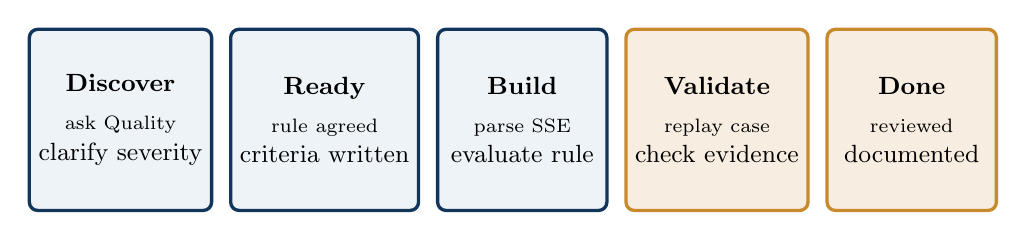
\begin{tikzpicture}[node distance=0.2cm]
\node[flowbox, minimum width=2.15cm, minimum height=2.3cm] (todo) {\textbf{Discover}\\[0.3em]\scriptsize ask Quality\\clarify severity};
\node[flowbox, minimum width=2.15cm, minimum height=2.3cm, right=of todo] (ready) {\textbf{Ready}\\[0.3em]\scriptsize rule agreed\\criteria written};
\node[flowbox, minimum width=2.15cm, minimum height=2.3cm, right=of ready] (build) {\textbf{Build}\\[0.3em]\scriptsize parse SSE\\evaluate rule};
\node[accentbox, minimum width=2.15cm, minimum height=2.3cm, right=of build] (valid) {\textbf{Validate}\\[0.3em]\scriptsize replay case\\check evidence};
\node[accentbox, minimum width=2.15cm, minimum height=2.3cm, right=of valid] (done) {\textbf{Done}\\[0.3em]\scriptsize reviewed\\documented};
\end{tikzpicture}
\vspace{0.5em}\begin{itemize}\item The board makes hidden requirements, documentation, and validation work visible instead of pretending every task is pure coding.\end{itemize}
\coursefooter
\end{frame}

\begin{frame}{Estimation is for coordination, not prediction theater}
\begin{itemize}
\item Story points work best as a relative complexity language shared by the team.
\item Estimation fails when people use points as disguised hours.
\item High-uncertainty tasks should often be split into investigation work before full implementation.
\item Velocity should guide planning, not evaluate people.
\end{itemize}
\coursefooter
\end{frame}

\begin{frame}{Frameworks and their natural use}
\begin{columns}[T]
\column{0.48\textwidth}\textbf{Structured rhythm}\begin{itemize}\item Scrum: bounded sprint goals, structured events and roles\item Good for student teams needing cadence and review moments\end{itemize}
\column{0.48\textwidth}\textbf{Flow orientation}\begin{itemize}\item Kanban: continuous incoming work, flow-oriented management\item Good for ops-heavy teams or highly varied work types\end{itemize}
\end{columns}
\vspace{0.5em}\begin{block}{Bridge}DevOps shares responsibility across build, release, and operations; MLOps extends it with data, models, drift, and governance concerns.\end{block}
\coursefooter
\end{frame}

\begin{frame}{Agile anti-patterns in data teams}
\begin{itemize}
\item Treating research uncertainty as ordinary feature implementation.
\item Filling sprints with vague work such as ``improve model'' or ``make dashboard better''.
\item Ignoring data dependencies until late integration.
\item Demonstrating only happy paths instead of operational evidence.
\item Identifying problems in retrospectives but never changing behavior.
\end{itemize}
\coursefooter
\end{frame}

\begin{frame}{What good agile behavior looks like in this course}
\repoactivity{\begin{itemize}
\item Demonstrate thin slices such as ingest plus one rule plus one alert rather than isolated fragments.
\item Keep boards aligned with requirements, deployment work, operational documentation, and validation.
\item Make uncertainty visible through investigation tasks, assumptions, and risks.
\item Show how stakeholder feedback changes backlog priorities instead of pretending the first plan was complete.
\end{itemize}}
\coursefooter
\end{frame}

\classclosingframe
{\begin{itemize}\item Agile in data-driven work means learning quickly while preserving evidence and alignment.\item Stories, boards, demos, and retrospectives are useful only when they reflect technical and data reality.\item Thin vertical slices are stronger than isolated notebook achievements.\end{itemize}}
{Teams should now be able to organize milestones, backlog items, and reviews around deployable progress instead of vague promises.}
{Class 35 connects this discipline to the project requirements and development plan.}
{Agile coordination gives the team a way to move continuously; sound engineering practices make that movement dependable.}

\begin{frame}{Papers and materials}
\readinglist{\href{https://www.scrumguides.org/}{Scrum Guide};\ \href{https://kanban.university/kanban-resources/getting-started/what-is-kanban/}{What is Kanban};\ \href{https://www.oreilly.com/library/view/learning-agile/9780596527679/}{Learning Agile};\ \href{https://martinfowler.com/bliki/UserStory.html}{Martin Fowler on user stories};\ \href{https://itrevolution.com/product/accelerate/}{Forsgren, Humble, Kim, Accelerate}.}
\coursefooter
\end{frame}
\end{document}
